\PassOptionsToPackage{unicode=true}{hyperref} % options for packages loaded elsewhere
\PassOptionsToPackage{hyphens}{url}
%
\documentclass[ignorenonframetext,]{beamer}
\usepackage{pgfpages}
\setbeamertemplate{caption}[numbered]
\setbeamertemplate{caption label separator}{: }
\setbeamercolor{caption name}{fg=normal text.fg}
\beamertemplatenavigationsymbolsempty
\usepackage{lmodern}
\usepackage{amssymb,amsmath}
\usepackage{ifxetex,ifluatex}
\usepackage{fixltx2e} % provides \textsubscript
\ifnum 0\ifxetex 1\fi\ifluatex 1\fi=0 % if pdftex
  \usepackage[T1]{fontenc}
  \usepackage[utf8]{inputenc}
  \usepackage{textcomp} % provides euro and other symbols
\else % if luatex or xelatex
  \usepackage{unicode-math}
  \defaultfontfeatures{Ligatures=TeX,Scale=MatchLowercase}
\fi
% use upquote if available, for straight quotes in verbatim environments
\IfFileExists{upquote.sty}{\usepackage{upquote}}{}
% use microtype if available
\IfFileExists{microtype.sty}{%
\usepackage[]{microtype}
\UseMicrotypeSet[protrusion]{basicmath} % disable protrusion for tt fonts
}{}
\IfFileExists{parskip.sty}{%
\usepackage{parskip}
}{% else
\setlength{\parindent}{0pt}
\setlength{\parskip}{6pt plus 2pt minus 1pt}
}
\usepackage{hyperref}
\hypersetup{
            pdftitle={A whirlwind tour of Rstudio, R, and Rmarkdown Magic for behavioral and brain scientists},
            pdfauthor={Jenny Rieck \& Derek Beaton},
            pdfborder={0 0 0},
            breaklinks=true}
\urlstyle{same}  % don't use monospace font for urls
\newif\ifbibliography
\usepackage{color}
\usepackage{fancyvrb}
\newcommand{\VerbBar}{|}
\newcommand{\VERB}{\Verb[commandchars=\\\{\}]}
\DefineVerbatimEnvironment{Highlighting}{Verbatim}{commandchars=\\\{\}}
% Add ',fontsize=\small' for more characters per line
\usepackage{framed}
\definecolor{shadecolor}{RGB}{248,248,248}
\newenvironment{Shaded}{\begin{snugshade}}{\end{snugshade}}
\newcommand{\AlertTok}[1]{\textcolor[rgb]{0.94,0.16,0.16}{#1}}
\newcommand{\AnnotationTok}[1]{\textcolor[rgb]{0.56,0.35,0.01}{\textbf{\textit{#1}}}}
\newcommand{\AttributeTok}[1]{\textcolor[rgb]{0.77,0.63,0.00}{#1}}
\newcommand{\BaseNTok}[1]{\textcolor[rgb]{0.00,0.00,0.81}{#1}}
\newcommand{\BuiltInTok}[1]{#1}
\newcommand{\CharTok}[1]{\textcolor[rgb]{0.31,0.60,0.02}{#1}}
\newcommand{\CommentTok}[1]{\textcolor[rgb]{0.56,0.35,0.01}{\textit{#1}}}
\newcommand{\CommentVarTok}[1]{\textcolor[rgb]{0.56,0.35,0.01}{\textbf{\textit{#1}}}}
\newcommand{\ConstantTok}[1]{\textcolor[rgb]{0.00,0.00,0.00}{#1}}
\newcommand{\ControlFlowTok}[1]{\textcolor[rgb]{0.13,0.29,0.53}{\textbf{#1}}}
\newcommand{\DataTypeTok}[1]{\textcolor[rgb]{0.13,0.29,0.53}{#1}}
\newcommand{\DecValTok}[1]{\textcolor[rgb]{0.00,0.00,0.81}{#1}}
\newcommand{\DocumentationTok}[1]{\textcolor[rgb]{0.56,0.35,0.01}{\textbf{\textit{#1}}}}
\newcommand{\ErrorTok}[1]{\textcolor[rgb]{0.64,0.00,0.00}{\textbf{#1}}}
\newcommand{\ExtensionTok}[1]{#1}
\newcommand{\FloatTok}[1]{\textcolor[rgb]{0.00,0.00,0.81}{#1}}
\newcommand{\FunctionTok}[1]{\textcolor[rgb]{0.00,0.00,0.00}{#1}}
\newcommand{\ImportTok}[1]{#1}
\newcommand{\InformationTok}[1]{\textcolor[rgb]{0.56,0.35,0.01}{\textbf{\textit{#1}}}}
\newcommand{\KeywordTok}[1]{\textcolor[rgb]{0.13,0.29,0.53}{\textbf{#1}}}
\newcommand{\NormalTok}[1]{#1}
\newcommand{\OperatorTok}[1]{\textcolor[rgb]{0.81,0.36,0.00}{\textbf{#1}}}
\newcommand{\OtherTok}[1]{\textcolor[rgb]{0.56,0.35,0.01}{#1}}
\newcommand{\PreprocessorTok}[1]{\textcolor[rgb]{0.56,0.35,0.01}{\textit{#1}}}
\newcommand{\RegionMarkerTok}[1]{#1}
\newcommand{\SpecialCharTok}[1]{\textcolor[rgb]{0.00,0.00,0.00}{#1}}
\newcommand{\SpecialStringTok}[1]{\textcolor[rgb]{0.31,0.60,0.02}{#1}}
\newcommand{\StringTok}[1]{\textcolor[rgb]{0.31,0.60,0.02}{#1}}
\newcommand{\VariableTok}[1]{\textcolor[rgb]{0.00,0.00,0.00}{#1}}
\newcommand{\VerbatimStringTok}[1]{\textcolor[rgb]{0.31,0.60,0.02}{#1}}
\newcommand{\WarningTok}[1]{\textcolor[rgb]{0.56,0.35,0.01}{\textbf{\textit{#1}}}}
\usepackage{graphicx,grffile}
\makeatletter
\def\maxwidth{\ifdim\Gin@nat@width>\linewidth\linewidth\else\Gin@nat@width\fi}
\def\maxheight{\ifdim\Gin@nat@height>\textheight\textheight\else\Gin@nat@height\fi}
\makeatother
% Scale images if necessary, so that they will not overflow the page
% margins by default, and it is still possible to overwrite the defaults
% using explicit options in \includegraphics[width, height, ...]{}
\setkeys{Gin}{width=\maxwidth,height=\maxheight,keepaspectratio}
% Prevent slide breaks in the middle of a paragraph:
\widowpenalties 1 10000
\raggedbottom
\setbeamertemplate{part page}{
\centering
\begin{beamercolorbox}[sep=16pt,center]{part title}
  \usebeamerfont{part title}\insertpart\par
\end{beamercolorbox}
}
\setbeamertemplate{section page}{
\centering
\begin{beamercolorbox}[sep=12pt,center]{part title}
  \usebeamerfont{section title}\insertsection\par
\end{beamercolorbox}
}
\setbeamertemplate{subsection page}{
\centering
\begin{beamercolorbox}[sep=8pt,center]{part title}
  \usebeamerfont{subsection title}\insertsubsection\par
\end{beamercolorbox}
}
\AtBeginPart{
  \frame{\partpage}
}
\AtBeginSection{
  \ifbibliography
  \else
    \frame{\sectionpage}
  \fi
}
\AtBeginSubsection{
  \frame{\subsectionpage}
}
\setlength{\emergencystretch}{3em}  % prevent overfull lines
\providecommand{\tightlist}{%
  \setlength{\itemsep}{0pt}\setlength{\parskip}{0pt}}
\setcounter{secnumdepth}{0}

% set default figure placement to htbp
\makeatletter
\def\fps@figure{htbp}
\makeatother

\usepackage{beamerthemeshadow}

\title{A whirlwind tour of Rstudio, R, and Rmarkdown Magic for behavioral and
brain scientists}
\author{Jenny Rieck \& Derek Beaton}
\date{May 17 2019}

\begin{document}
\frame{\titlepage}

\begin{frame}{The big outline}
\protect\hypertarget{the-big-outline}{}

\begin{itemize}
\tightlist
\item
  Part 0: Background and Community
\item
  Part 1: Rstudio
\item
  Part 2: Project and environment setup
\item
  Part 3: R (et al., eg Python)
\item
  Part 4: Rmarkdown
\item
  Part 5: Advanced R and beyond
\item
  Part 6: A few of our favorite things
\end{itemize}

\end{frame}

\hypertarget{part-0-background-and-community}{%
\section{Part 0: Background and
Community}\label{part-0-background-and-community}}

\begin{frame}{Part 0: Background and Community}
\protect\hypertarget{part-0-background-and-community-1}{}

\begin{itemize}
\tightlist
\item
  What this is \& isn't; a bunch of things we aren't covering but you
  should be aware of

  \begin{itemize}
  \tightlist
  \item
    This is a taste and to bring you into a bigger world
  \end{itemize}
\item
  Centralization, standards
\item
  Help
\item
  Including rigor \& reproducibility of packages
\item
  The ``tidyverse''

  \begin{itemize}
  \tightlist
  \item
    Learn it. But don't learn \emph{only} the tidyverse; you'll be lost
    in base R
  \end{itemize}
\end{itemize}

\end{frame}

\begin{frame}{R Background}
\protect\hypertarget{r-background}{}

\begin{itemize}
\tightlist
\item
  Created in 1992 by Gentleman \& Ihaka
\end{itemize}

\emph{{[}we{]} considered the problem of obtaining decent statistical
software for our undergraduate Macintosh lab. After considering the
options, we decided that the most satisfactory alternative was to write
our own. {[}\ldots{}{]} Finally we added some syntactic sugar to make it
look somewhat like S. We call the result ``R''.}

\end{frame}

\begin{frame}{What is R?}
\protect\hypertarget{what-is-r}{}

\begin{itemize}
\tightlist
\item
  R is for stats and general purpose programming
\item
  R is a functional language

  \begin{itemize}
  \tightlist
  \item
    Turing complete -- can do anything other languages can do
  \end{itemize}
\item
  R is an environment to inferface with the langauge

  \begin{itemize}
  \tightlist
  \item
    Console based
  \item
    Type in commands
  \item
    No point-and-click
  \end{itemize}
\item
  R is a collection of tools

  \begin{itemize}
  \tightlist
  \item
    Pre-packaged software at your disposal
  \end{itemize}
\item
  R is free (as in beer and speech)

  \begin{itemize}
  \tightlist
  \item
    No cost, no restrictions
  \end{itemize}
\end{itemize}

\end{frame}

\begin{frame}{R is a bit ugly}
\protect\hypertarget{r-is-a-bit-ugly}{}

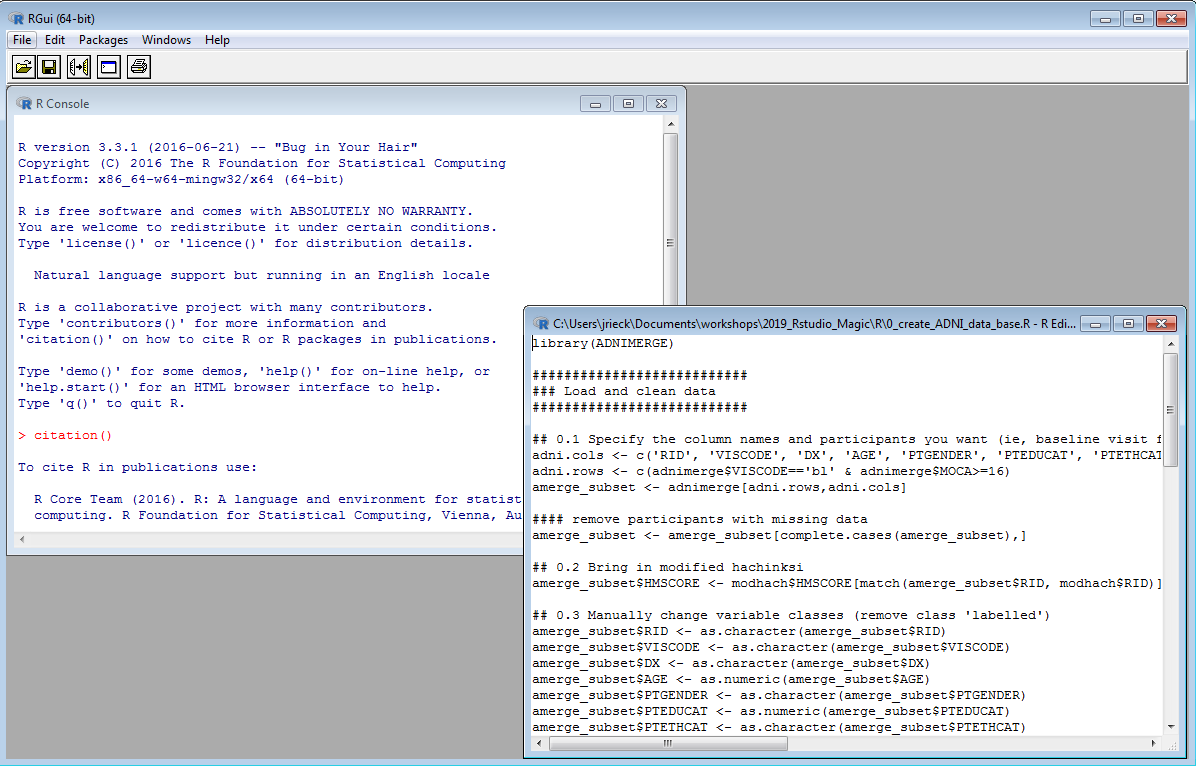
\includegraphics{../external/images/intro_rgui.PNG}

\end{frame}

\begin{frame}{But R has many interfaces}
\protect\hypertarget{but-r-has-many-interfaces}{}

\begin{itemize}
\tightlist
\item
  Today we focus on RStudio (MatLab-like)
\item
  But see also Deducer, RCommander (SPSS-like)
  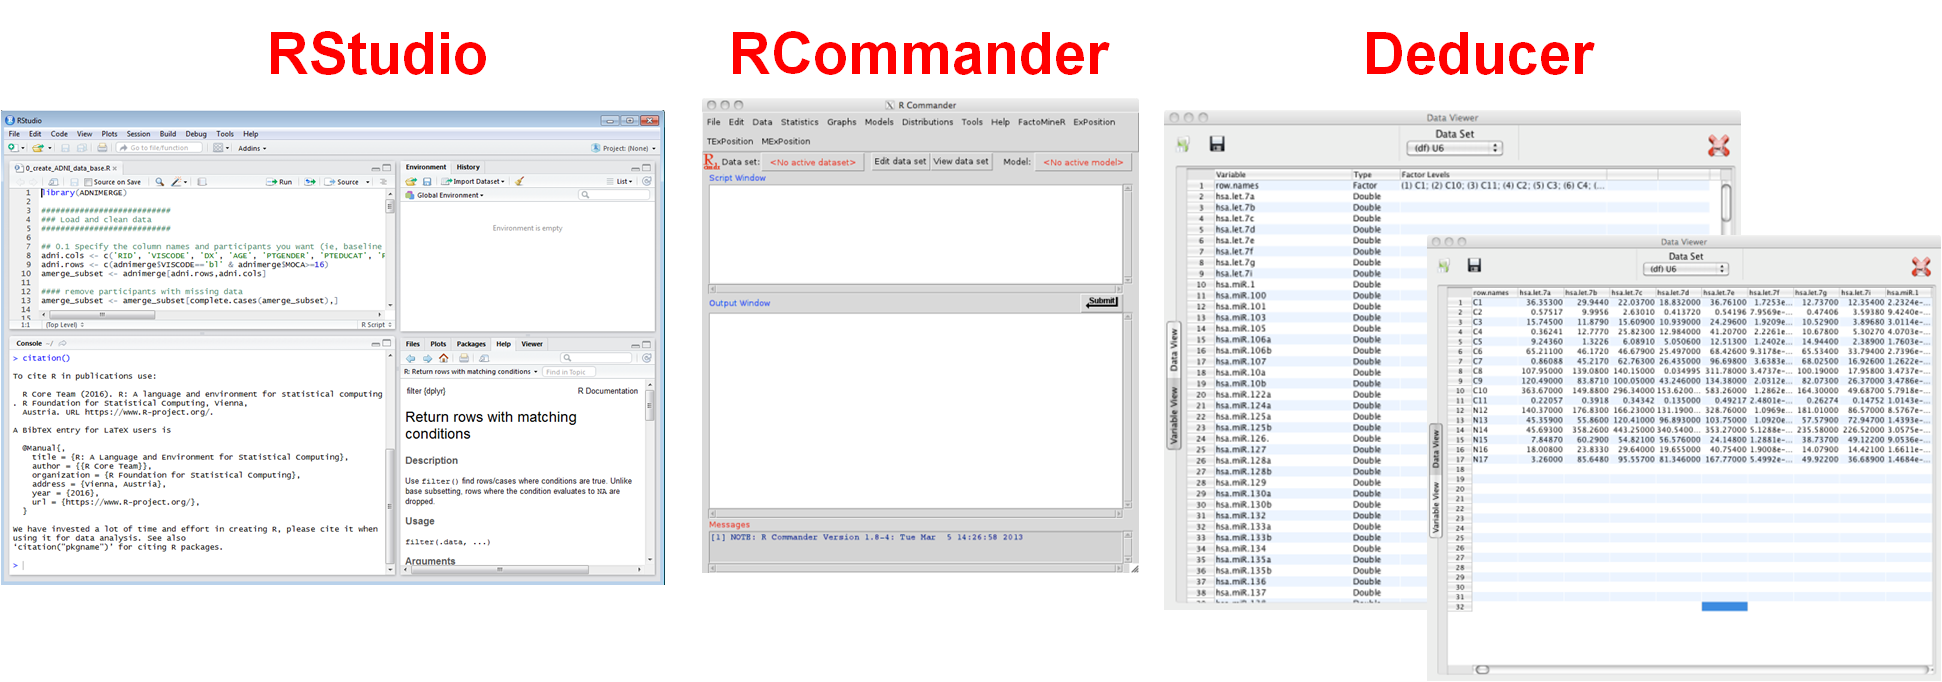
\includegraphics{../external/images/intro_rgui_2.PNG}
\end{itemize}

\end{frame}

\begin{frame}{R is a community (actually many communities!)}
\protect\hypertarget{r-is-a-community-actually-many-communities}{}

\begin{itemize}
\tightlist
\item
  Help and resources
\item
  Package development and distribution
\end{itemize}

\end{frame}

\begin{frame}{R: Help!}
\protect\hypertarget{r-help}{}

\begin{itemize}
\tightlist
\item
  \url{https://www.statmethods.net/}
\item
  Online forums (Stack Exchange, r-lists)
\item
  SpringerLink

  \begin{itemize}
  \tightlist
  \item
    All R books for free (pdf format) or for minimal cost (printed)
  \end{itemize}
\item
  Vignettes

  \begin{itemize}
  \tightlist
  \item
    step-by-step instruction guides for packages
  \end{itemize}
\end{itemize}

\end{frame}

\begin{frame}{R Packages}
\protect\hypertarget{r-packages}{}

\begin{itemize}
\tightlist
\item
  Packages are bundles of code made by someone (or many people) for
  everyone to use

  \begin{itemize}
  \tightlist
  \item
    If you can think of a stats problem, there is a package for it
  \end{itemize}
\item
  Available primarily on CRAN

  \begin{itemize}
  \tightlist
  \item
    But also github, r-forge
  \end{itemize}
\end{itemize}

\end{frame}

\begin{frame}{Tidyverse}
\protect\hypertarget{tidyverse}{}

\begin{itemize}
\tightlist
\item
  something here about tidy
\end{itemize}

\end{frame}

\hypertarget{part-1-rstudio}{%
\section{Part 1: Rstudio}\label{part-1-rstudio}}

\begin{frame}{Part 1: RStudio}
\protect\hypertarget{part-1-rstudio-1}{}

\begin{itemize}
\tightlist
\item
  Settings, a quit tour through stuff, features
\item
  Examples on getting setup
\end{itemize}

\end{frame}

\begin{frame}{RStudio Environment}
\protect\hypertarget{rstudio-environment}{}

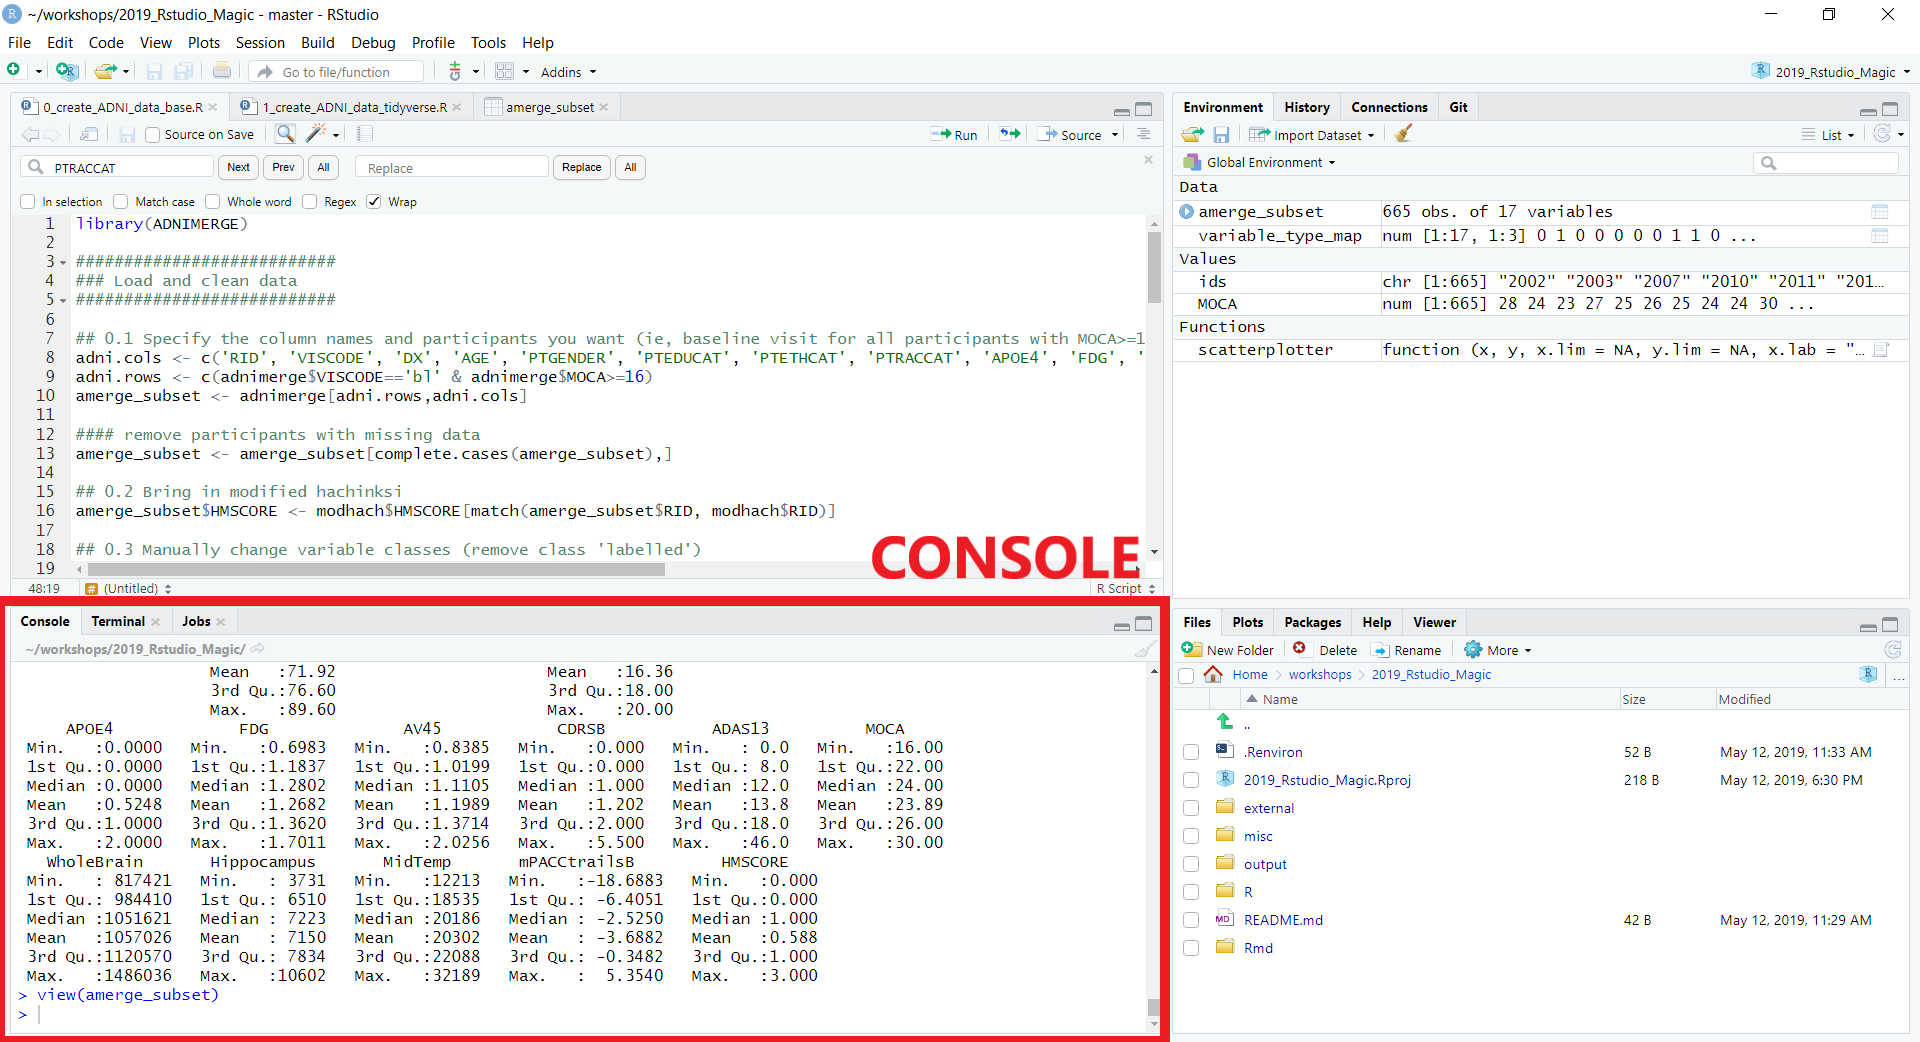
\includegraphics{../external/images/rstudio_terminal_1_CONSOLE.png}

\end{frame}

\begin{frame}{RStudio Environment}
\protect\hypertarget{rstudio-environment-1}{}

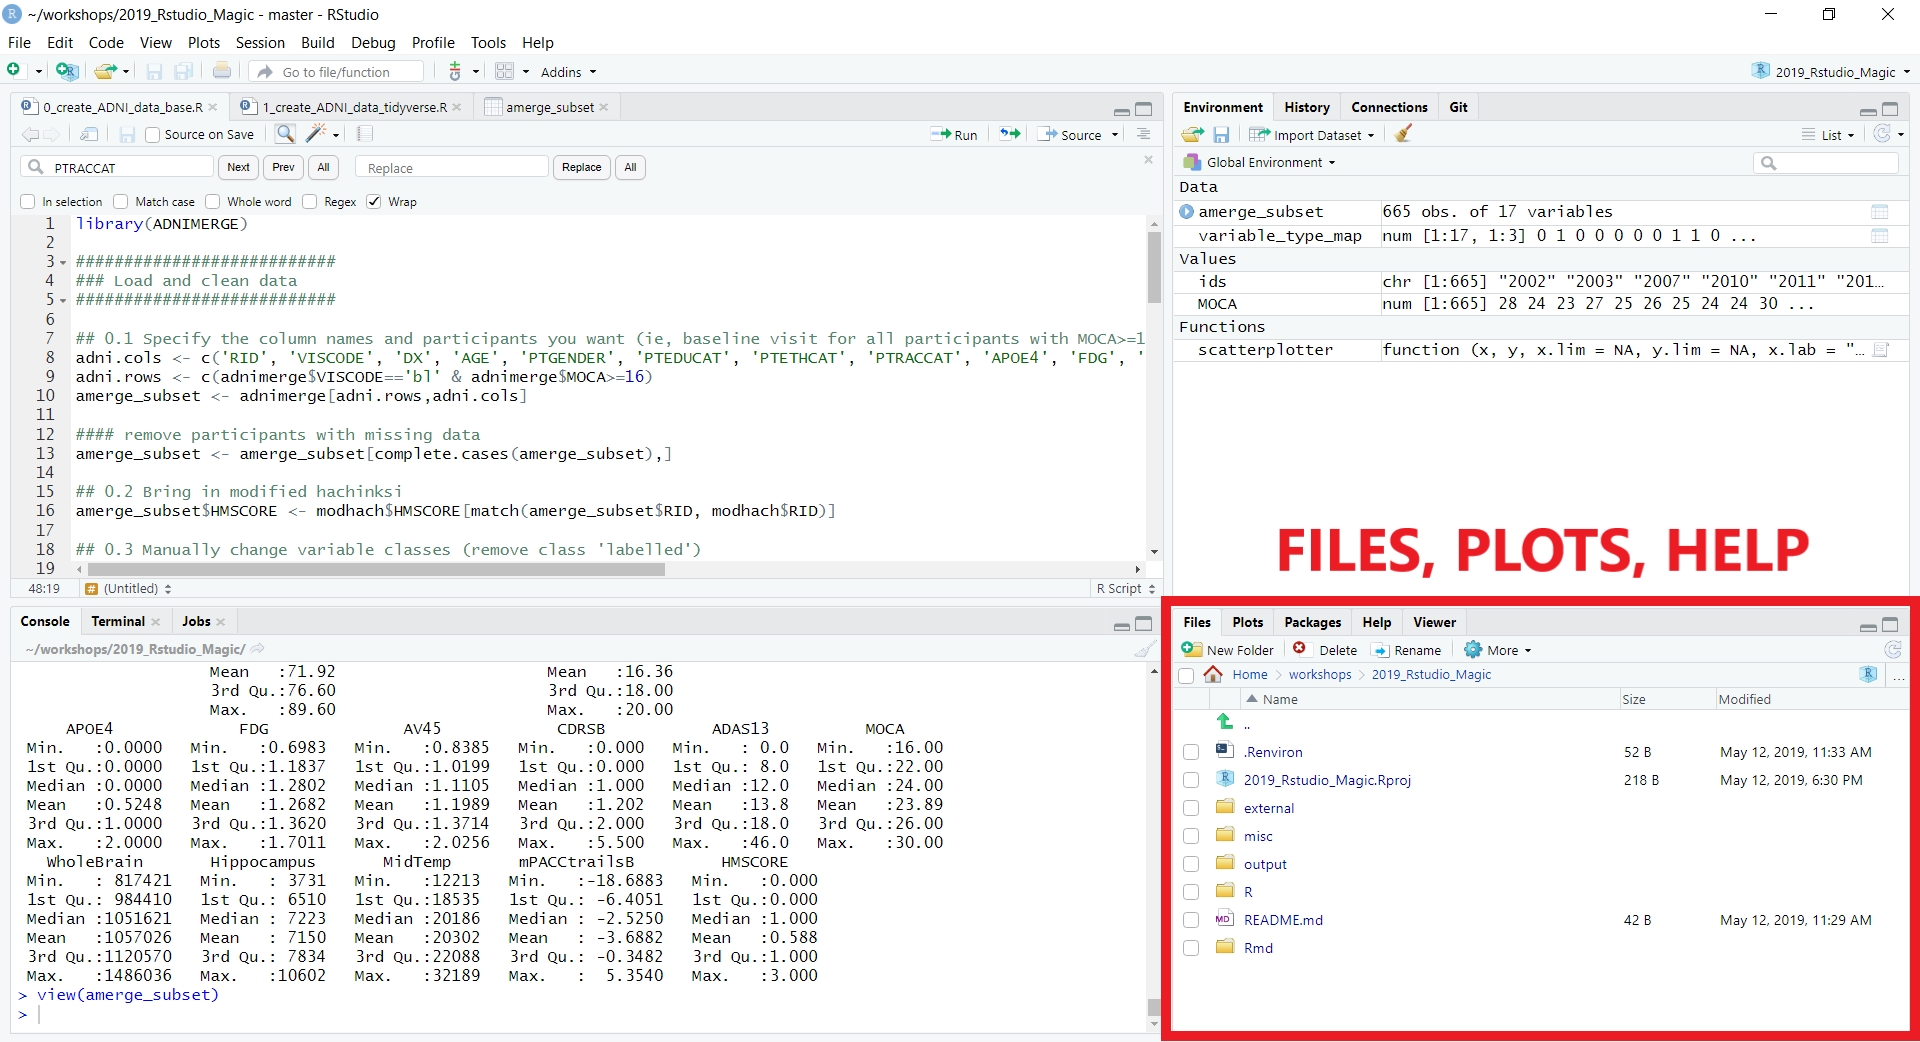
\includegraphics{../external/images/rstudio_terminal_2_FILES.png}

\end{frame}

\begin{frame}{RStudio Environment}
\protect\hypertarget{rstudio-environment-2}{}

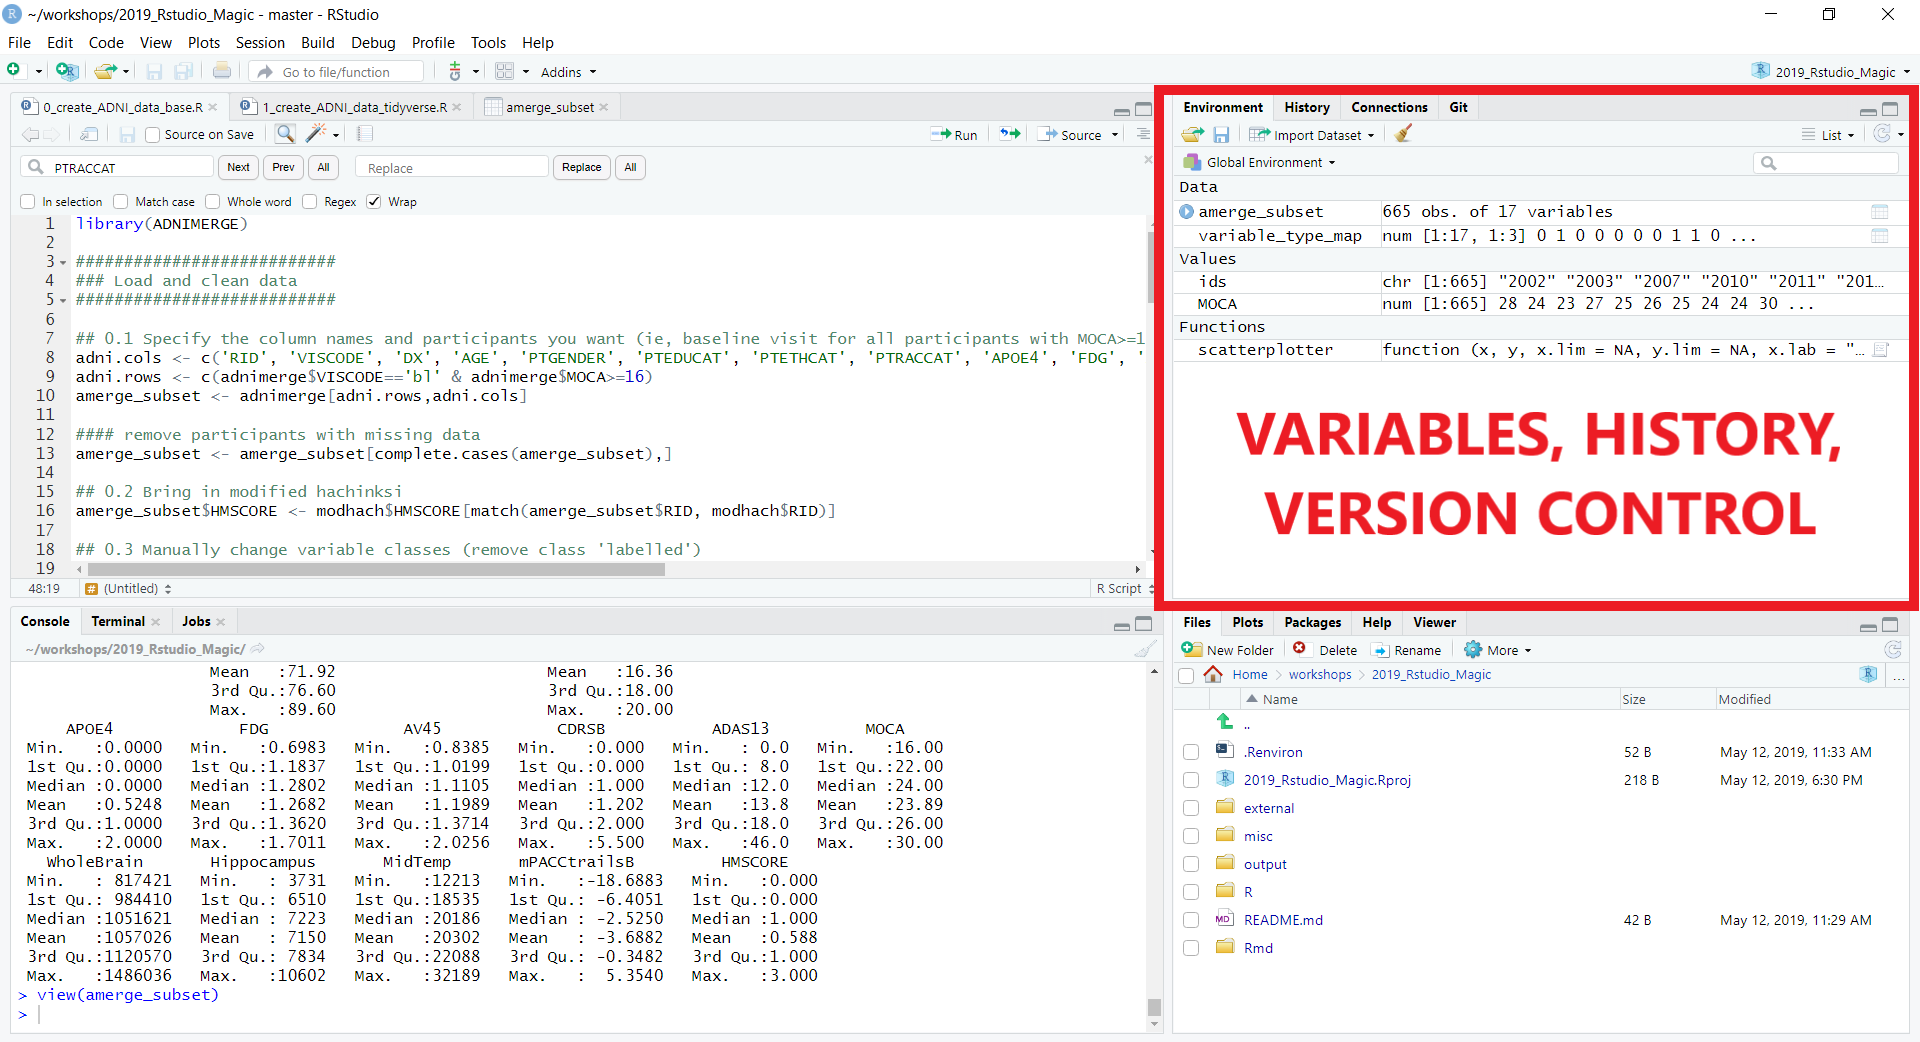
\includegraphics{../external/images/rstudio_terminal_3_ENV.png}

\end{frame}

\begin{frame}{RStudio Environment}
\protect\hypertarget{rstudio-environment-3}{}

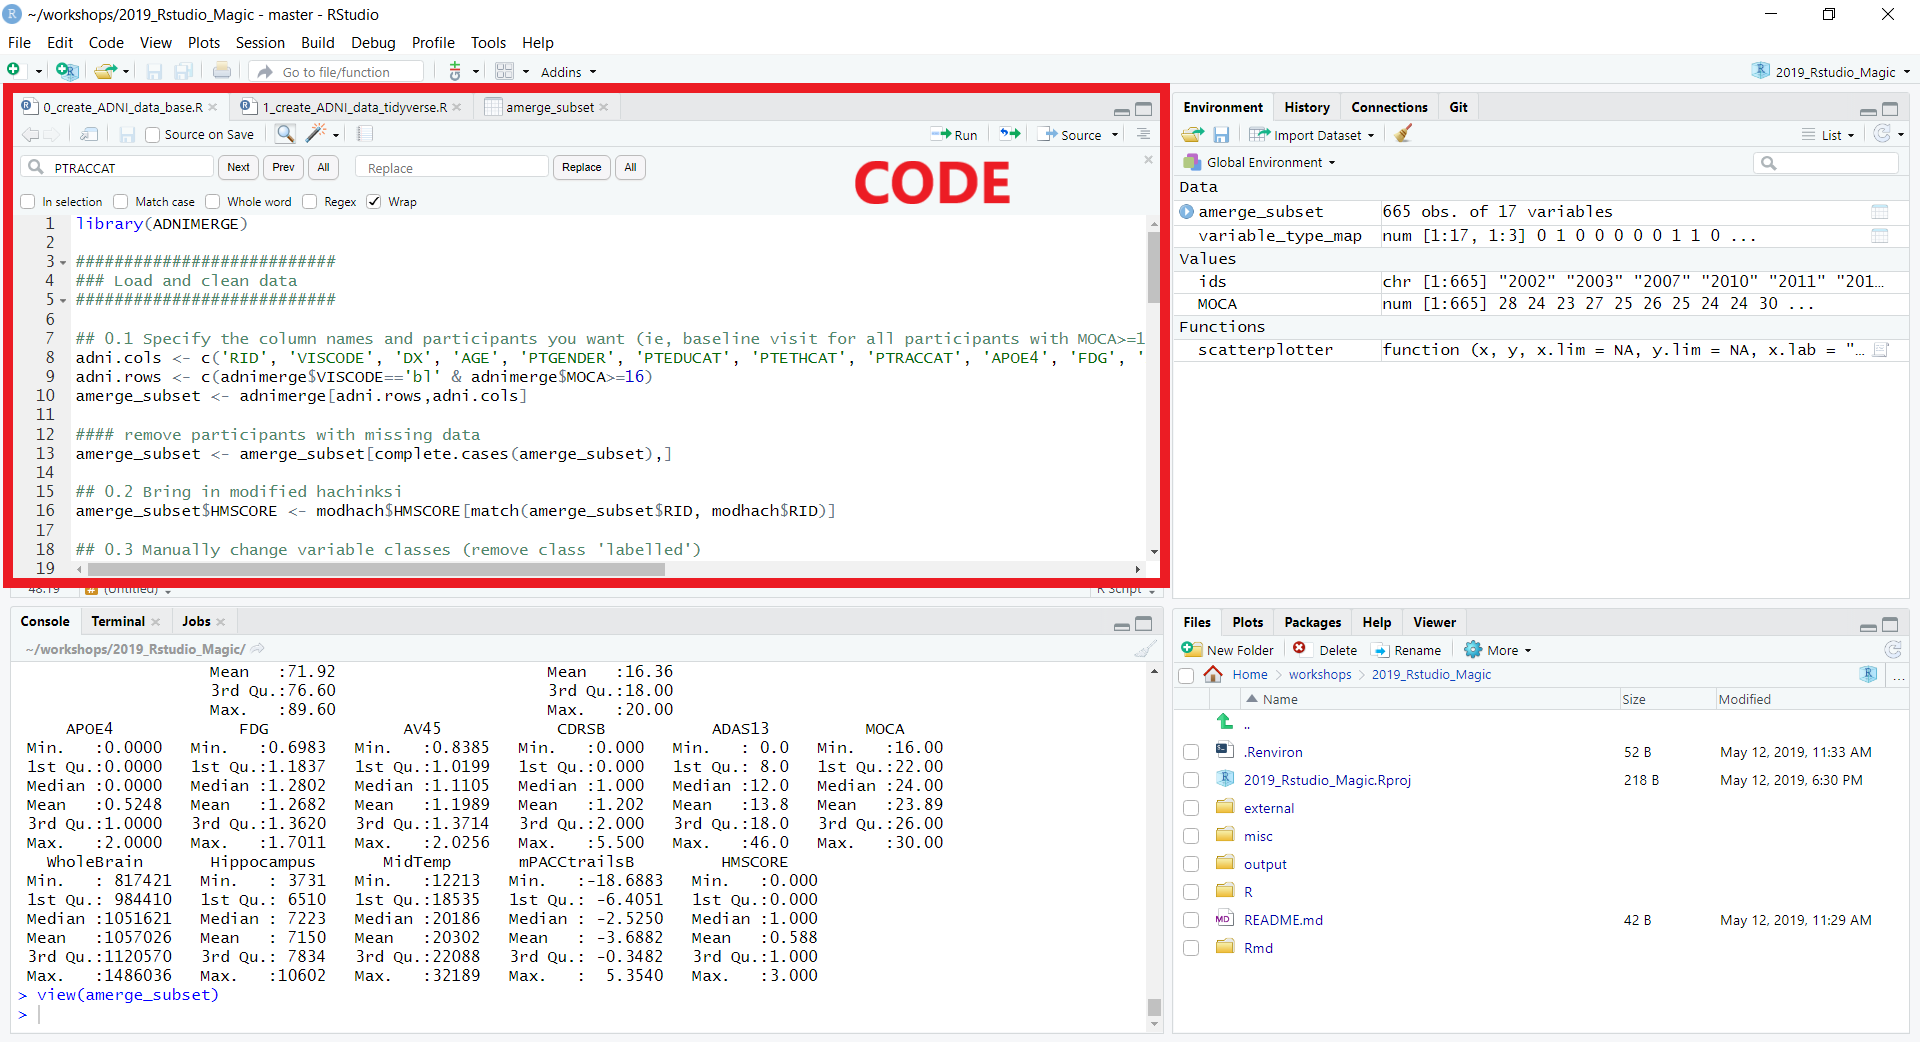
\includegraphics{../external/images/rstudio_terminal_4_CODE.png}

\end{frame}

\begin{frame}{RStudio Environment}
\protect\hypertarget{rstudio-environment-4}{}

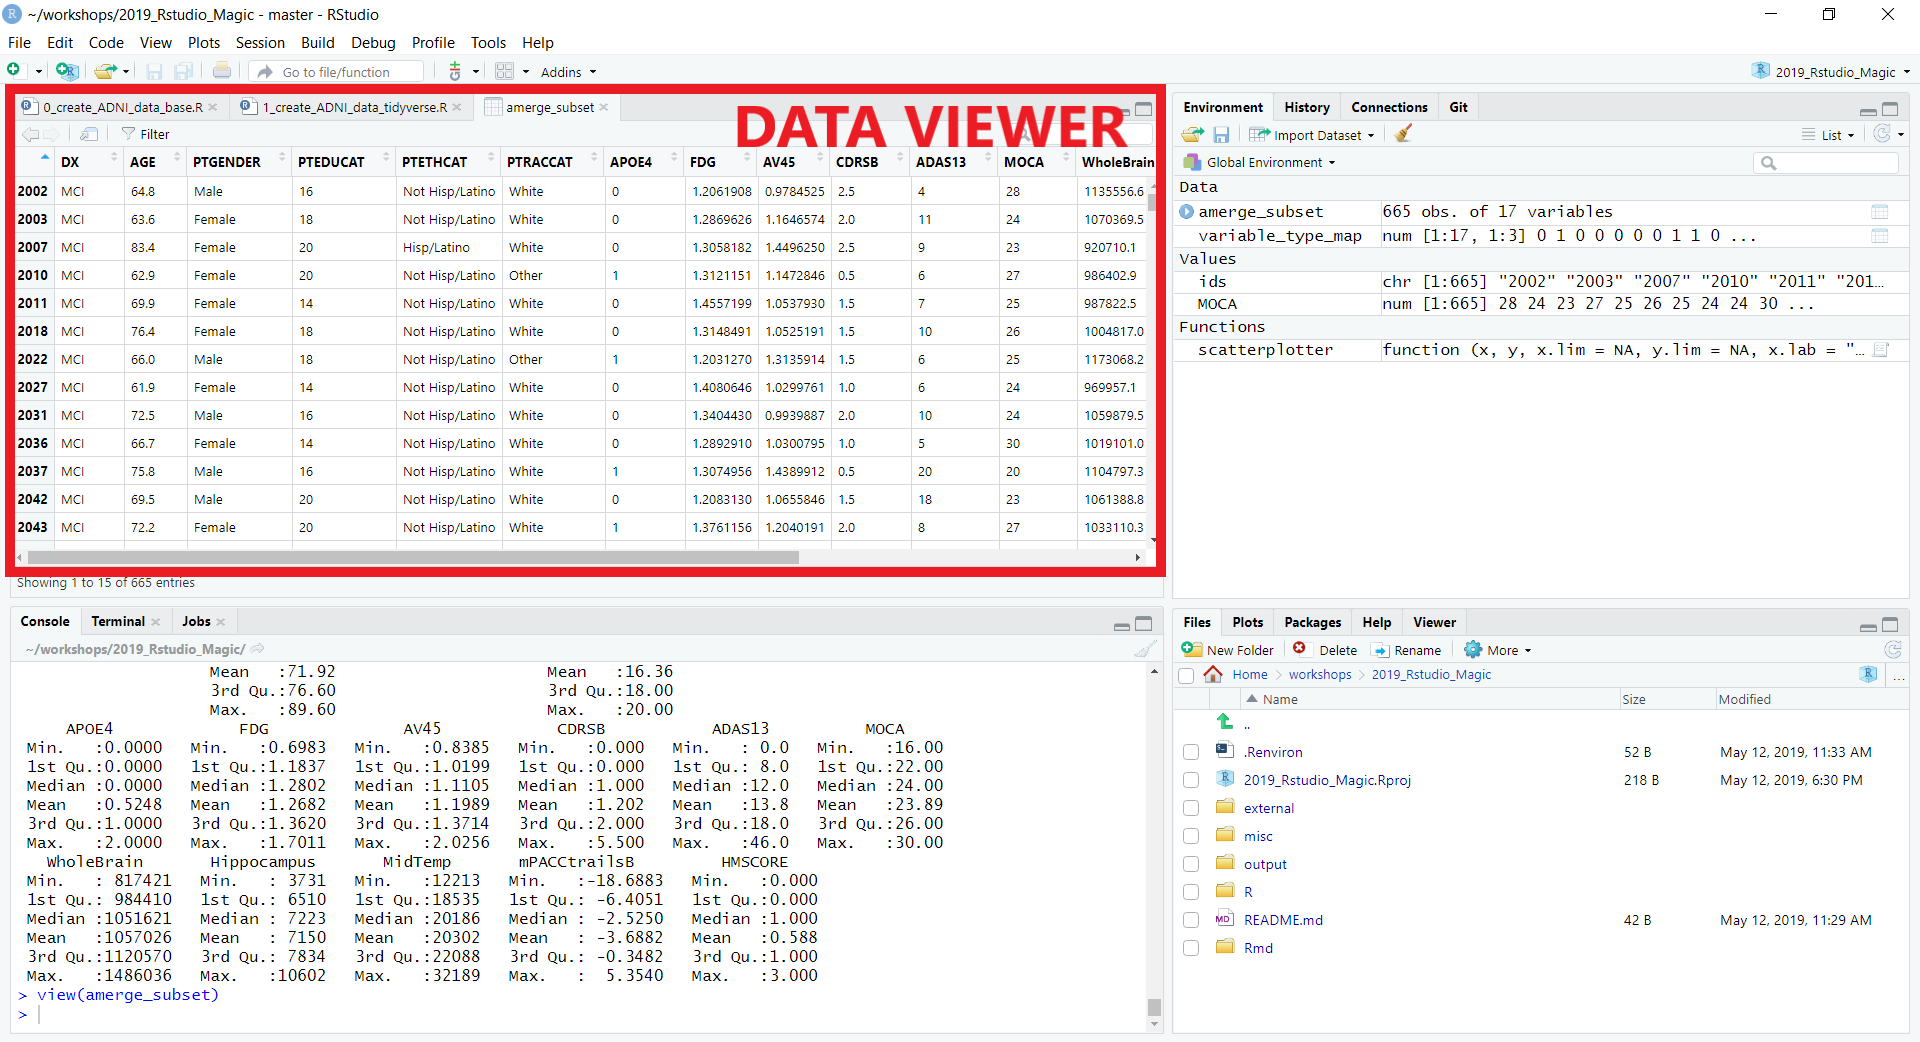
\includegraphics{../external/images/rstudio_terminal_5_DATA.png}

\end{frame}

\begin{frame}{Benefits of RStudio}
\protect\hypertarget{benefits-of-rstudio}{}

\begin{itemize}
\tightlist
\item
  Built-in integration with version control (git or SVN)
\item
  Package and documentation generation
\item
  Reproducible science!

  \begin{itemize}
  \tightlist
  \item
    R Markdown documents

    \begin{itemize}
    \tightlist
    \item
      Save and execute code
    \item
      Generate high quality reports that can be shared
    \end{itemize}
  \item
    Create presentations (like this one!)
  \item
    Even write papers
  \end{itemize}
\end{itemize}

\end{frame}

\begin{frame}{RStudio Resources}
\protect\hypertarget{rstudio-resources}{}

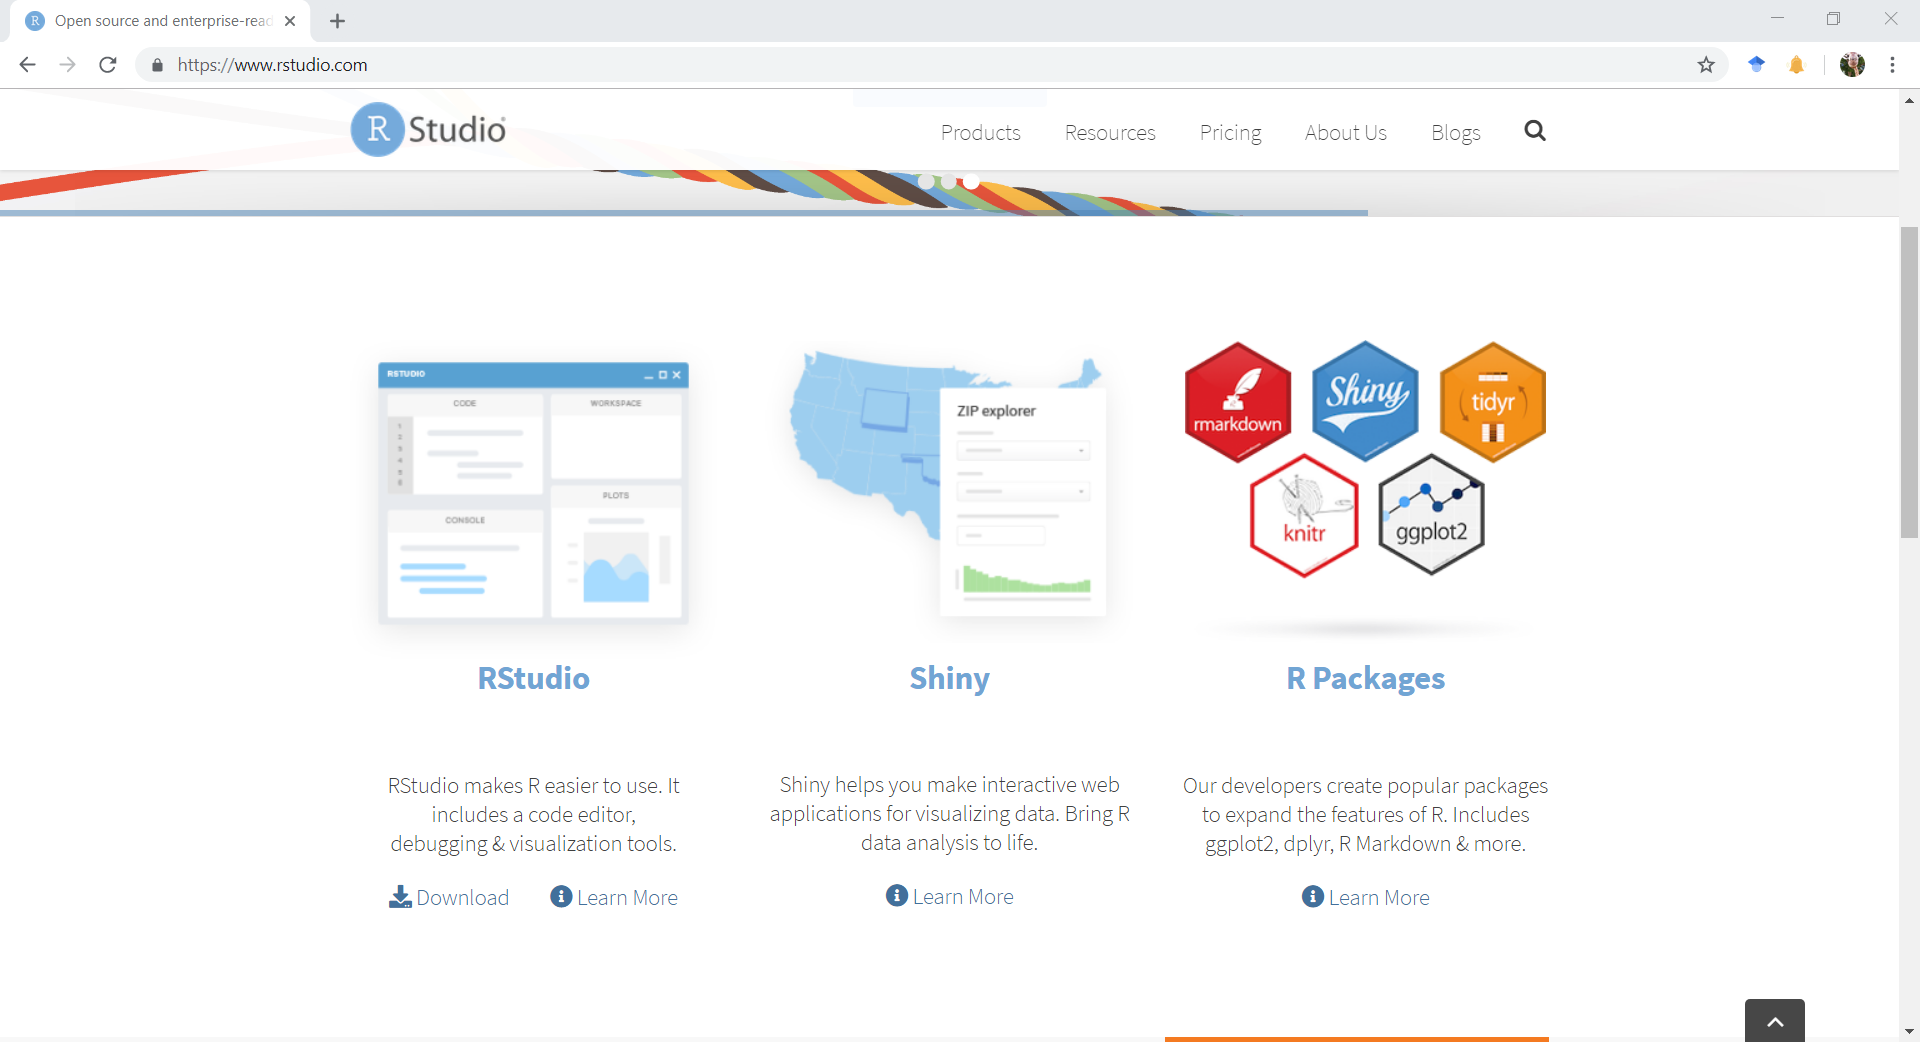
\includegraphics{../external/images/rstudio_dot_com_1_main.PNG}

\end{frame}

\begin{frame}{RStudio Resources}
\protect\hypertarget{rstudio-resources-1}{}

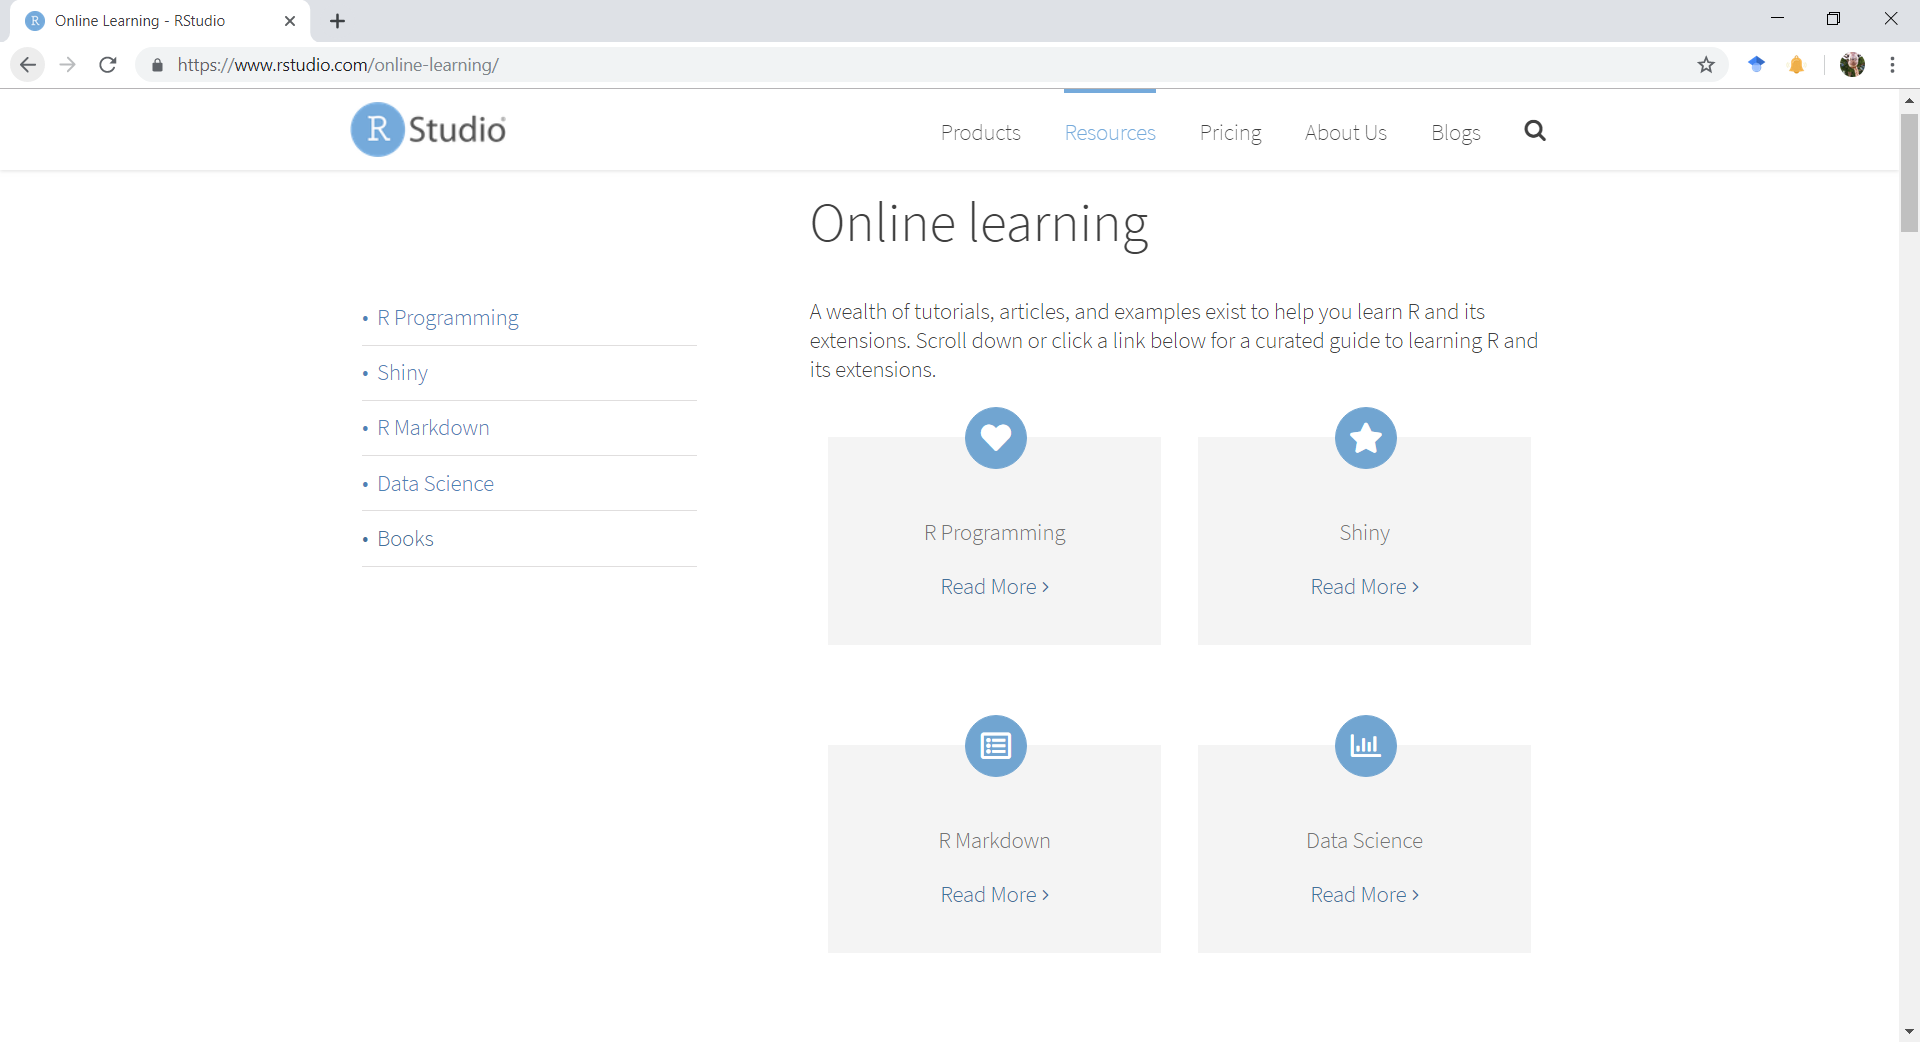
\includegraphics{../external/images/rstudio_dot_com_2_learning.PNG}

\end{frame}

\begin{frame}{RStudio Resources}
\protect\hypertarget{rstudio-resources-2}{}

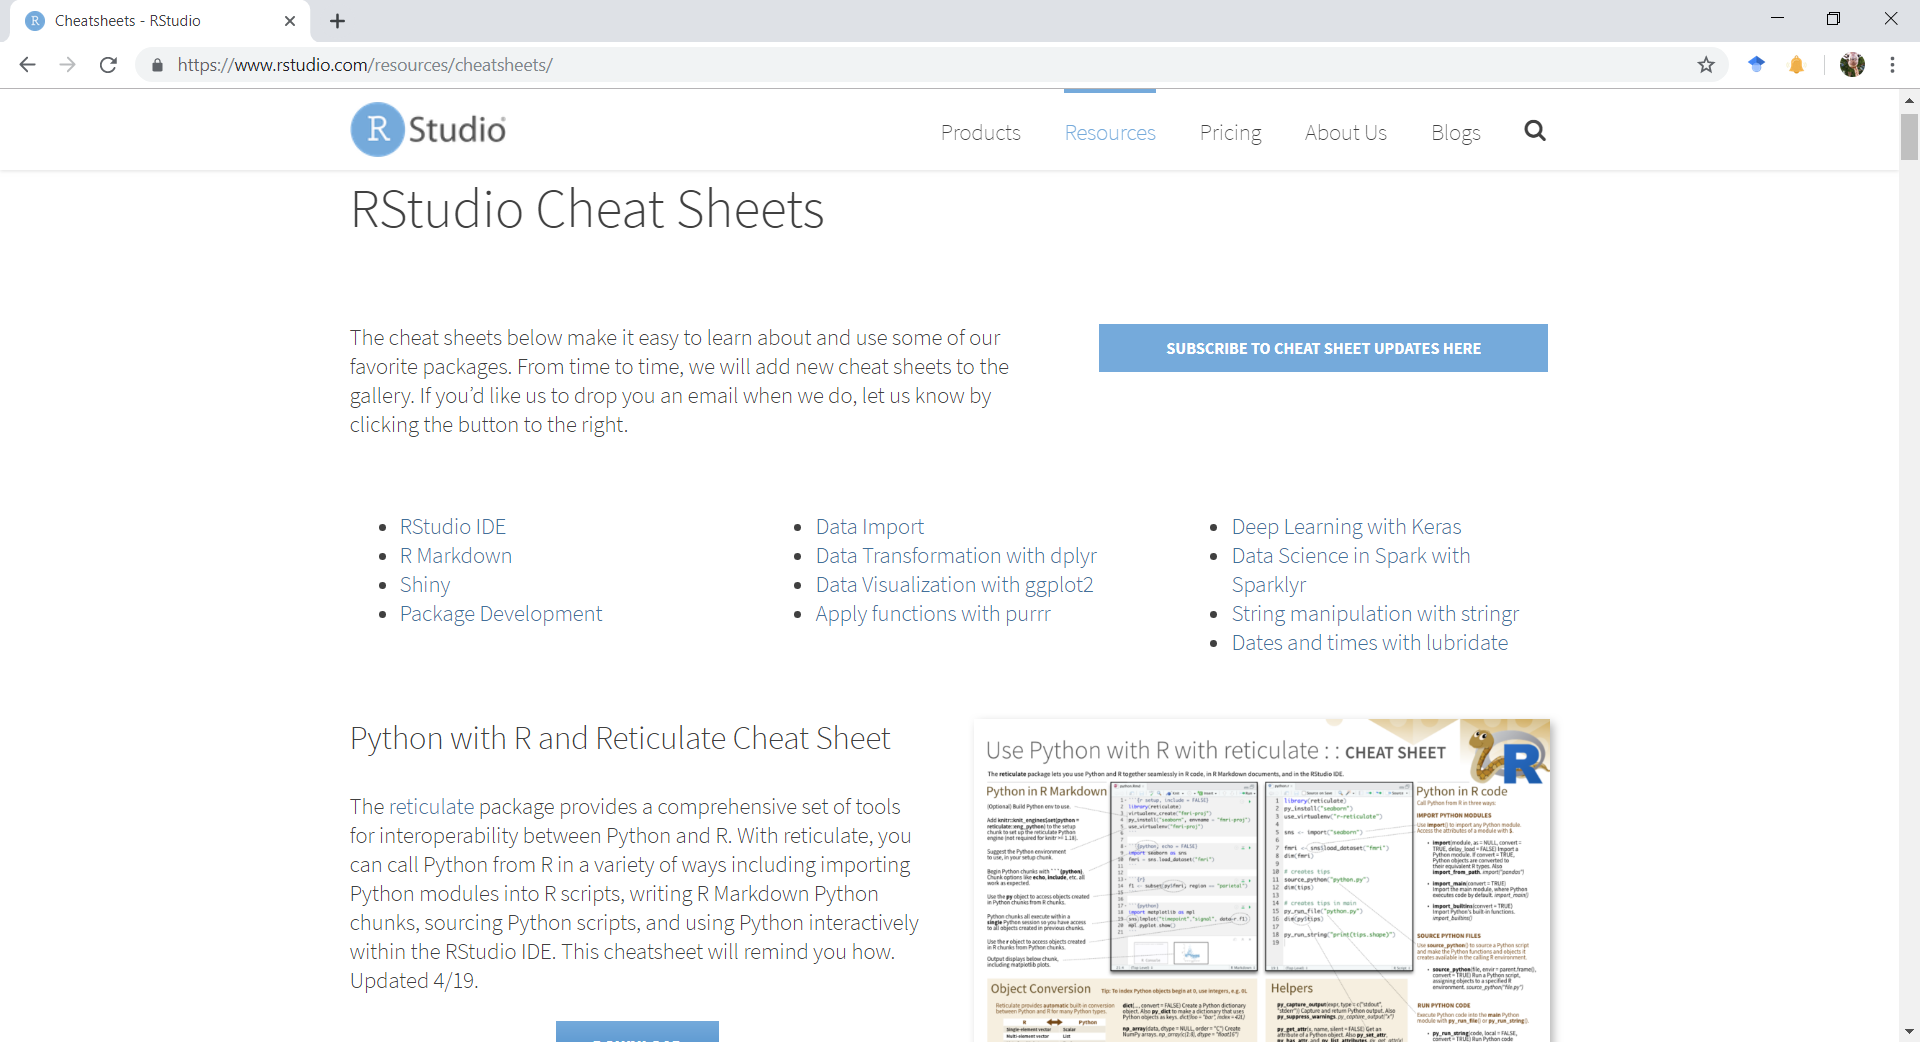
\includegraphics{../external/images/rstudio_dot_com_3_cheats.PNG}

\end{frame}

\hypertarget{part-2-setup}{%
\section{Part 2: Setup}\label{part-2-setup}}

\begin{frame}{Part 2: Project and Environment Setup}
\protect\hypertarget{part-2-project-and-environment-setup}{}

\begin{itemize}
\tightlist
\item
  Hidden files \& whatnot
\item
  Have a structure ready to go on Github
\item
  Explain/walk through
\item
  Discuss the helpful packages above
\end{itemize}

\end{frame}

\begin{frame}[fragile]{RStudio Setup}
\protect\hypertarget{rstudio-setup}{}

\begin{itemize}
\tightlist
\item
  Download R and Rstudio
\item
  Add-on packages
\end{itemize}

\begin{Shaded}
\begin{Highlighting}[]
\CommentTok{#to install from CRAN}
\KeywordTok{install.pacakges}\NormalTok{(}\StringTok{'devtools'}\NormalTok{, }\DataTypeTok{depenedencies =} \OtherTok{TRUE}\NormalTok{)}
\CommentTok{#to install from a file}
\KeywordTok{install.packages}\NormalTok{(}\StringTok{'/mypath/to/package/ADNIMERGE.tar.gz'}\NormalTok{, }
                 \DataTypeTok{type=}\StringTok{'source'}\NormalTok{, }\DataTypeTok{repos=}\OtherTok{NULL}\NormalTok{) }
\CommentTok{#to install from a git  (requires the devtools package)}
\NormalTok{dev.tools}\OperatorTok{::}\KeywordTok{install_github}\NormalTok{(Gibbsdavidl}\OperatorTok{/}\NormalTok{CatterPlots) }
\end{Highlighting}
\end{Shaded}

\begin{itemize}
\tightlist
\item
  See \url{https://jennybc.github.io/2014-05-12-ubc/r-setup.html} for a
  detailed guide
\end{itemize}

\end{frame}

\begin{frame}{Rstudio Setup: Projects \& Git}
\protect\hypertarget{rstudio-setup-projects-git}{}

\begin{itemize}
\tightlist
\item
  Download git and link to RStudio
  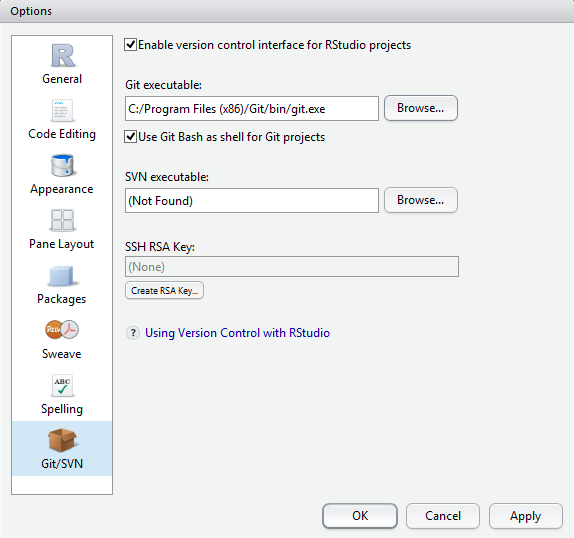
\includegraphics[width=0.75\textwidth,height=\textheight]{../external/images/setup_1_rstudio_git.PNG}
\end{itemize}

\end{frame}

\begin{frame}{Rstudio Setup: Projects \& Git}
\protect\hypertarget{rstudio-setup-projects-git-1}{}

\begin{itemize}
\tightlist
\item
  Create a new project File
  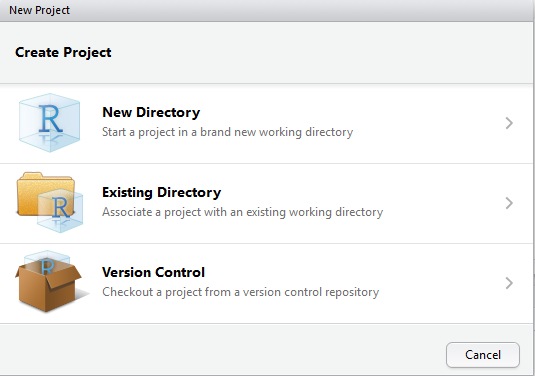
\includegraphics[width=0.75\textwidth,height=\textheight]{../external/images/setup_2_rstudio_project.PNG}
\end{itemize}

\end{frame}

\begin{frame}[fragile]{Format .gitignore}
\protect\hypertarget{format-.gitignore}{}

\begin{itemize}
\tightlist
\item
  File types to ignore:

  \begin{itemize}
  \tightlist
  \item
    \texttt{.Rproj.user}
  \item
    \texttt{.Rhistory}
  \item
    \texttt{.Ruserdata}
  \item
    \texttt{.Renviron}
  \item
    \texttt{.rda} \& \texttt{.Rdata} (to avoid pushing potentially
    sensitive data files to git)
  \item
    \texttt{**} before each extentions will match directories anywhere
    in the repo
  \end{itemize}
\end{itemize}

\end{frame}

\begin{frame}[fragile]{Format environmental variables}
\protect\hypertarget{format-environmental-variables}{}

\begin{itemize}
\tightlist
\item
  Set environmental variables (ie, directory location of data) to make
  code generalizable across computers

  \begin{itemize}
  \tightlist
  \item
    In your project folder create a \texttt{.Renviron} file and define
    variables
  \end{itemize}
\end{itemize}

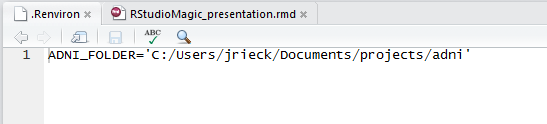
\includegraphics{../external/images/setup_3_rstudio_project_environ.PNG}

\end{frame}

\begin{frame}{Organize your project folders and markdown}
\protect\hypertarget{organize-your-project-folders-and-markdown}{}

*\url{https://emilyriederer.netlify.com/post/rmarkdown-driven-development/}
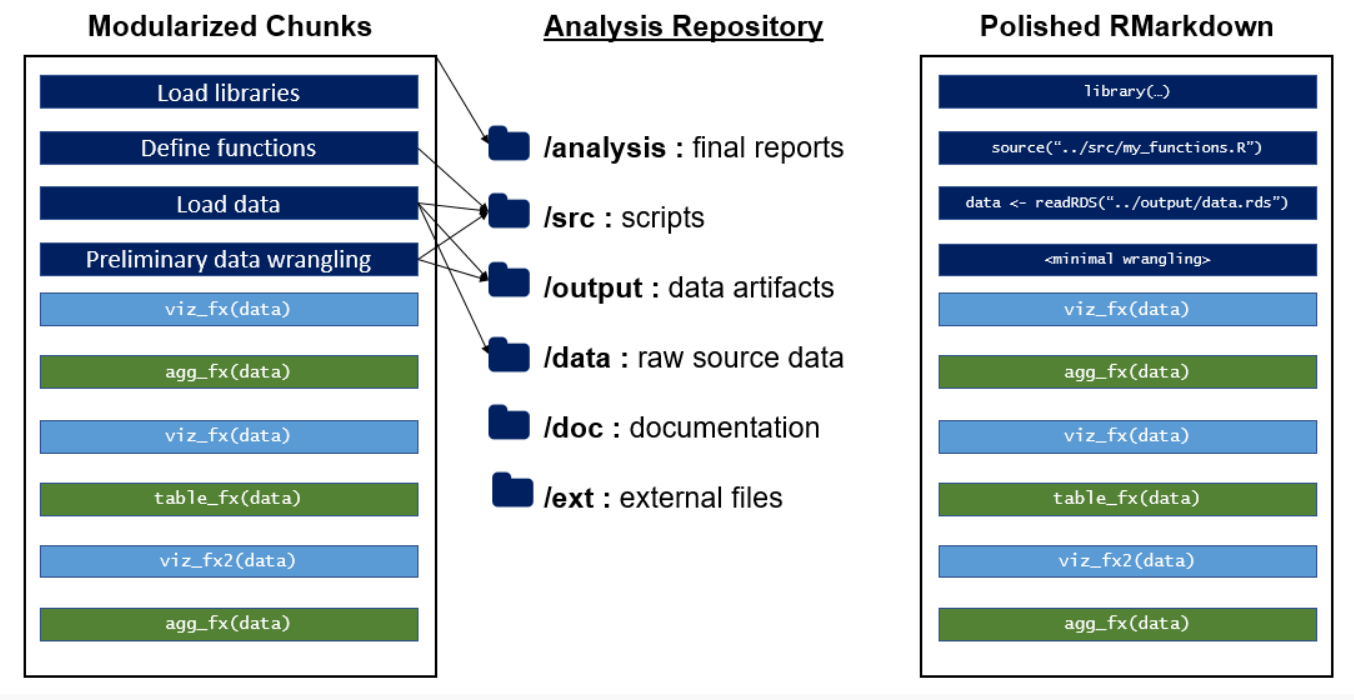
\includegraphics{../external/images/setup_4_markdown_project.PNG}

\end{frame}

\begin{frame}{Organize your project folders and markdown}
\protect\hypertarget{organize-your-project-folders-and-markdown-1}{}

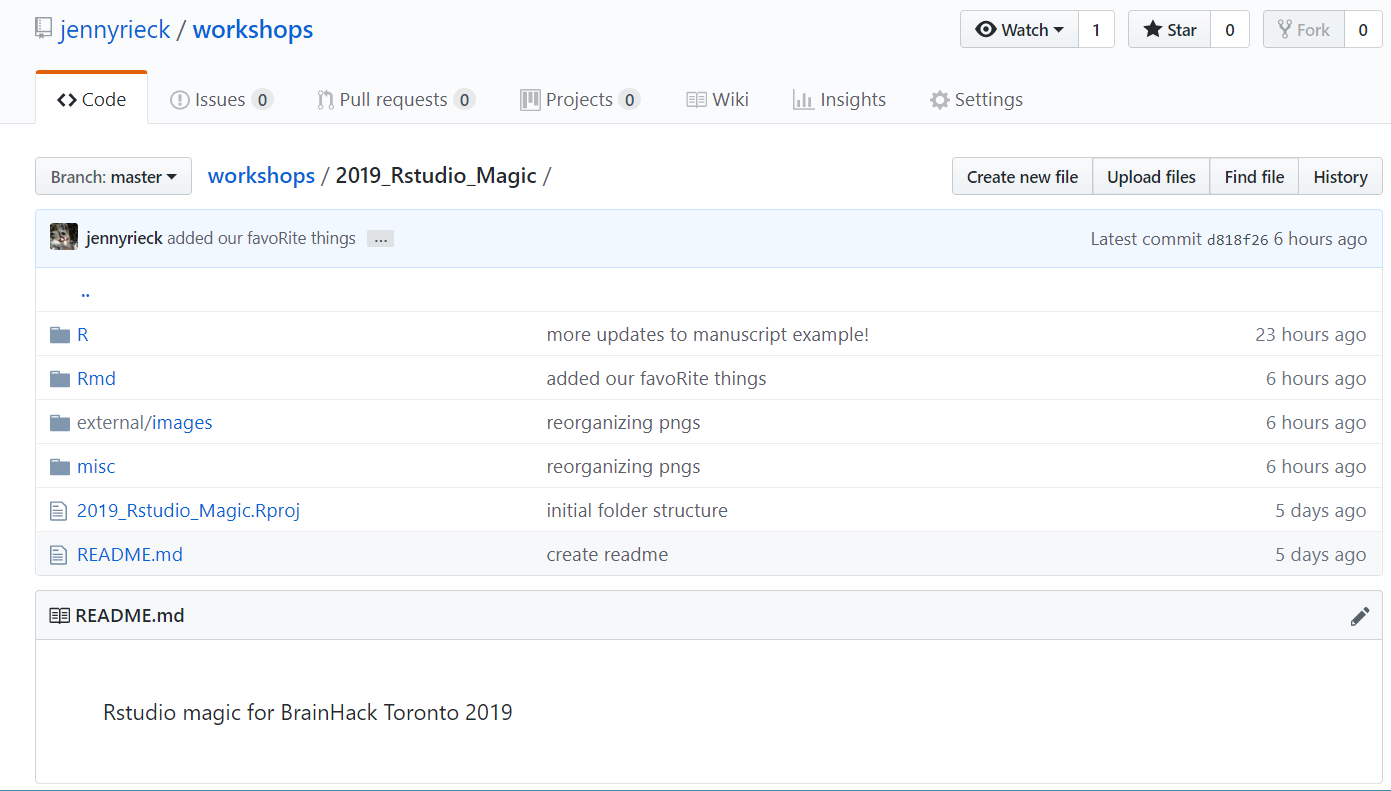
\includegraphics{../external/images/setup_5_git.PNG}

\end{frame}

\hypertarget{part-3-r-et-al}{%
\section{Part 3: R et al}\label{part-3-r-et-al}}

\begin{frame}{Part 3: R et al}
\protect\hypertarget{part-3-r-et-al-1}{}

\begin{itemize}
\tightlist
\item
  A bit of background, including idiosyncrasies and unique things about
  R

  \begin{itemize}
  \tightlist
  \item
    Especially packages \& three ways to install (somehwhat covered
    above) CRAN, Locally, Git \& others (devtools)
  \item
    It's a functional language
  \item
    Data types Including data frames \& alts like tibbles
  \end{itemize}
\item
  Read/explore

  \begin{itemize}
  \tightlist
  \item
    explore .R scripts
  \end{itemize}
\item
  Clean/export

  \begin{itemize}
  \tightlist
  \item
    Show 0\_Create from PCA/MCA with Base, Tidyverse, Plyr (NOT dplyr),
    data.table
  \item
    Reimport?
  \item
    Analyze With MCA \& covstatis
  \end{itemize}
\end{itemize}

\end{frame}

\hypertarget{part-4-rmarkdown}{%
\section{Part 4: RMarkdown}\label{part-4-rmarkdown}}

\begin{frame}{Part 4: RMarkdown}
\protect\hypertarget{part-4-rmarkdown-1}{}

\begin{itemize}
\tightlist
\item
  What it is /why to use it
\item
  A short deviation for LaTeX, and new helpers: kable \& kableExtra

  \begin{itemize}
  \tightlist
  \item
    A taxonomy and how to approach this \emph{Tying it all together
    through here 1: simple RMD }Plot-based visuals

    \begin{itemize}
    \tightlist
    \item
      Base, gt, ggplot, grobTable()/grid/gridExtra
    \item
      2: Slides (these ones here)
    \item
      3: Manuscripts!!
    \end{itemize}
  \end{itemize}
\item
  Reporting/presentin
\end{itemize}

\end{frame}

\hypertarget{part-5-advanced-r}{%
\section{Part 5: Advanced R}\label{part-5-advanced-r}}

\begin{frame}{Part 5: Some advanced/other things we're not covering}
\protect\hypertarget{part-5-some-advancedother-things-were-not-covering}{}

\begin{itemize}
\tightlist
\item
  package development
\item
  Shiny
\item
  SQL
\item
  C/C++
\item
  R2D3
\end{itemize}

\end{frame}

\hypertarget{part-6-extras}{%
\section{Part 6: Extras}\label{part-6-extras}}

\begin{frame}{Part 6: A few of our favorite things}
\protect\hypertarget{part-6-a-few-of-our-favorite-things}{}

\begin{itemize}
\tightlist
\item
  Fun R do-dads
\end{itemize}

\end{frame}

\begin{frame}[fragile]{CatterPlot for feline based graphics:}
\protect\hypertarget{catterplot-for-feline-based-graphics}{}

\begin{itemize}
\tightlist
\item
  \url{https://github.com/Gibbsdavidl/CatterPlots}
\end{itemize}

\texttt{dev.tools::install\_github(Gibbsdavidl/CatterPlots)}

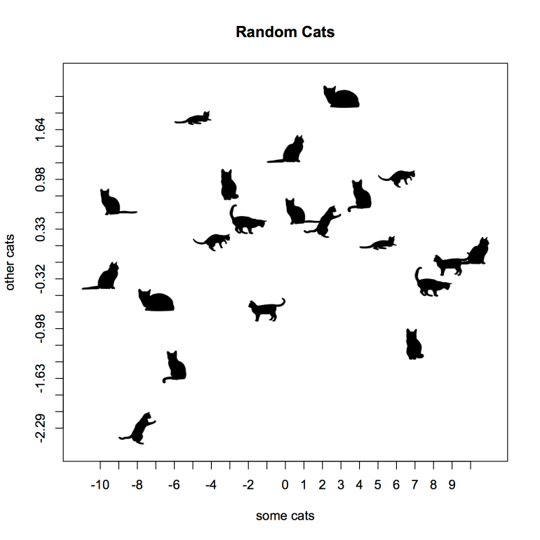
\includegraphics[width=0.6\textwidth,height=\textheight]{../external/images/funR_1_catterplotter.png}

\end{frame}

\begin{frame}[fragile]{What's a pirate's favorite programming language?}
\protect\hypertarget{whats-a-pirates-favorite-programming-language}{}

\begin{itemize}
\tightlist
\item
  \url{https://cran.r-project.org/web/packages/yarrr/vignettes/pirateplot.html}
\end{itemize}

\texttt{install.packages(\textquotesingle{}yarrr\textquotesingle{})}

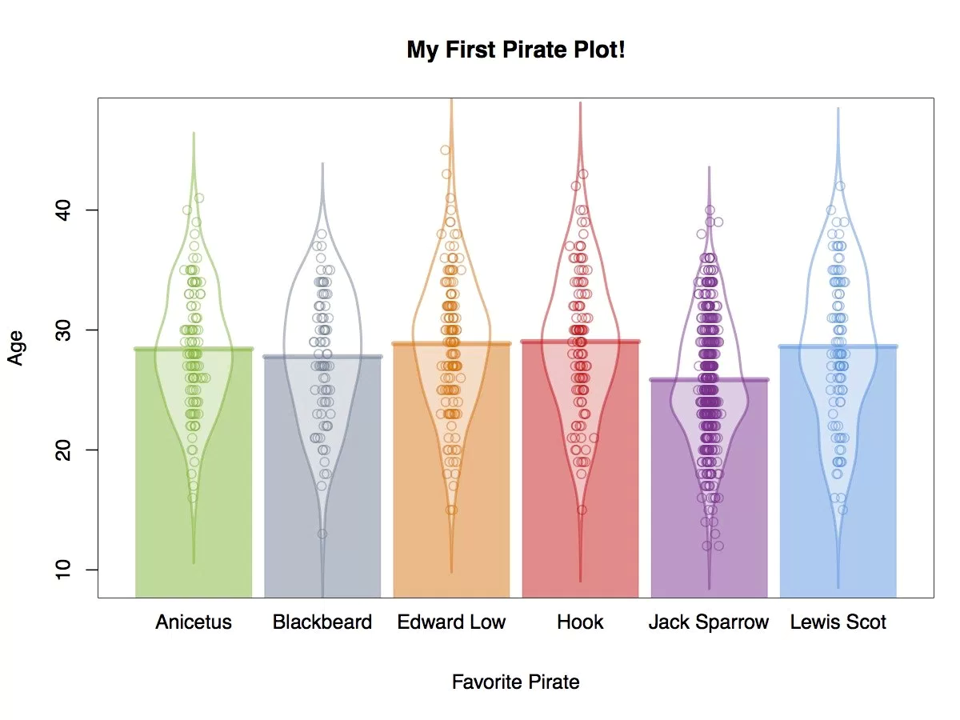
\includegraphics[width=0.75\textwidth,height=\textheight]{../external/images/funR_2_pirate.png}

\end{frame}

\begin{frame}[fragile]{Color palettes to fit your \textsubscript{mood}}
\protect\hypertarget{color-palettes-to-fit-your-mood}{}

\begin{itemize}
\tightlist
\item
  \url{https://github.com/karthik/wesanderson}
\end{itemize}

\texttt{dev.tools::install\_github(karthik/wesanderson)}

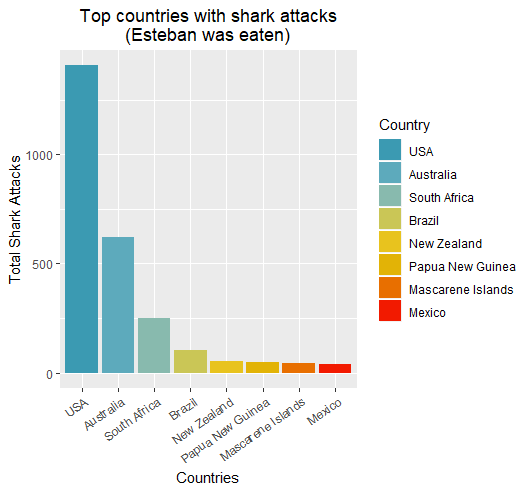
\includegraphics{../external/images/funR_3_wes_anderson.png}

\end{frame}

\begin{frame}[fragile]{Mapping your Strava routes}
\protect\hypertarget{mapping-your-strava-routes}{}

\begin{itemize}
\tightlist
\item
  \url{https://www.r-bloggers.com/strava-rides-map-in-r/}
\item
  ALSO \url{https://marcusvolz.com/?p=4068}

  \begin{itemize}
  \tightlist
  \item
    \texttt{dev.tools::install\_github(marcusvolz/strava)}
  \end{itemize}
\end{itemize}

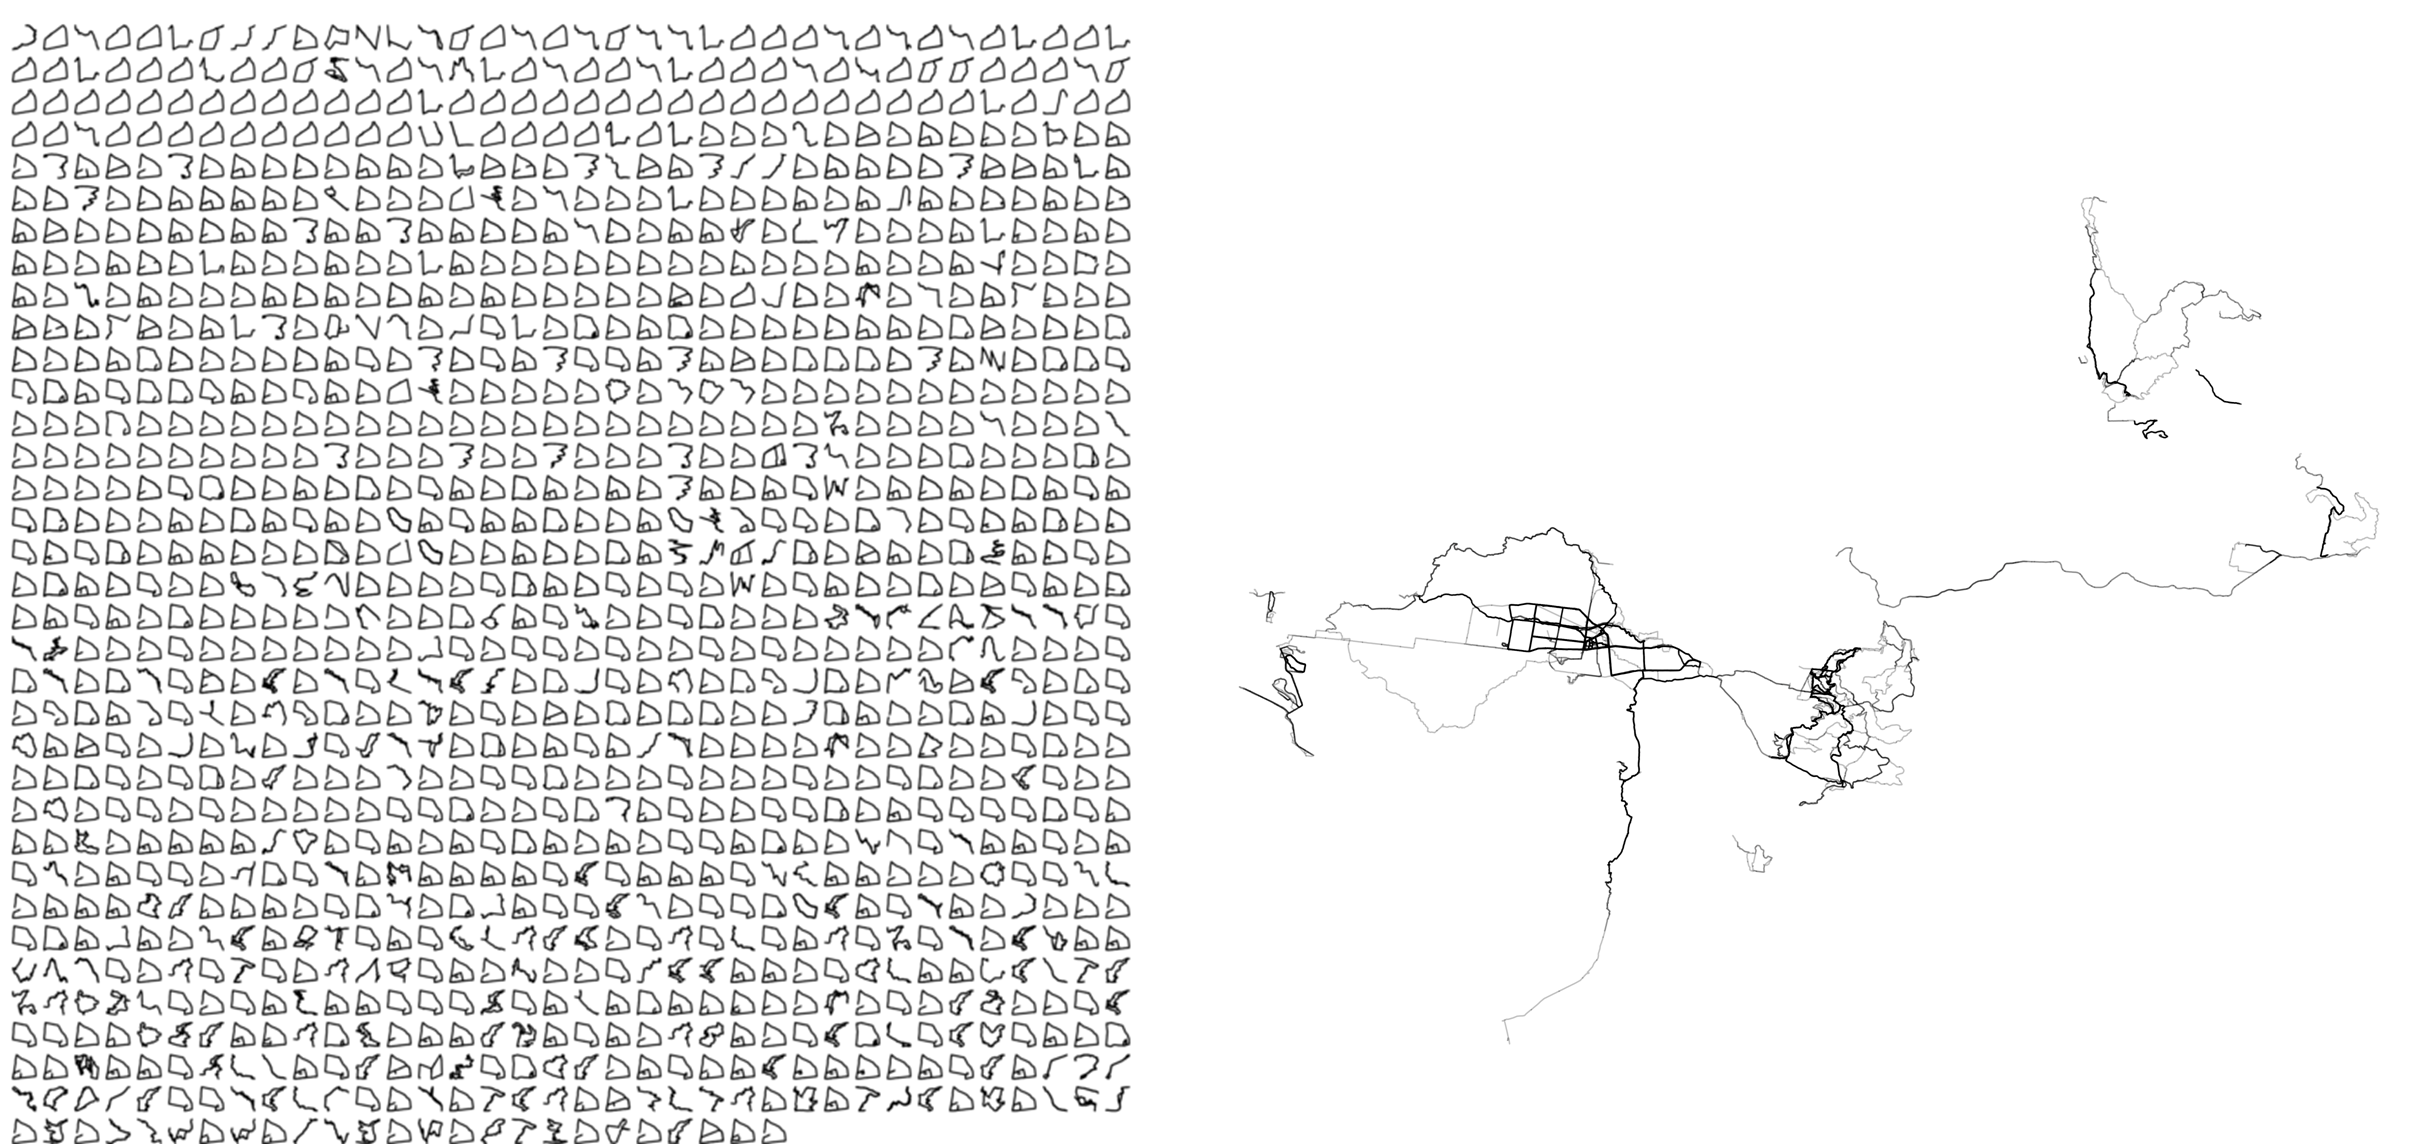
\includegraphics{../external/images/funR_4_strava_combo.png}

\end{frame}

\begin{frame}{Make aRt!}
\protect\hypertarget{make-art}{}

\begin{itemize}
\tightlist
\item
  R Graph Gallery

  \begin{itemize}
  \tightlist
  \item
    \url{http://www.r-graph-gallery.com/}
  \end{itemize}
\item
  Rtist: Gaston Sanchez

  \begin{itemize}
  \tightlist
  \item
    \url{http://gastonsanchez.com/Rtist/}
  \end{itemize}
\end{itemize}

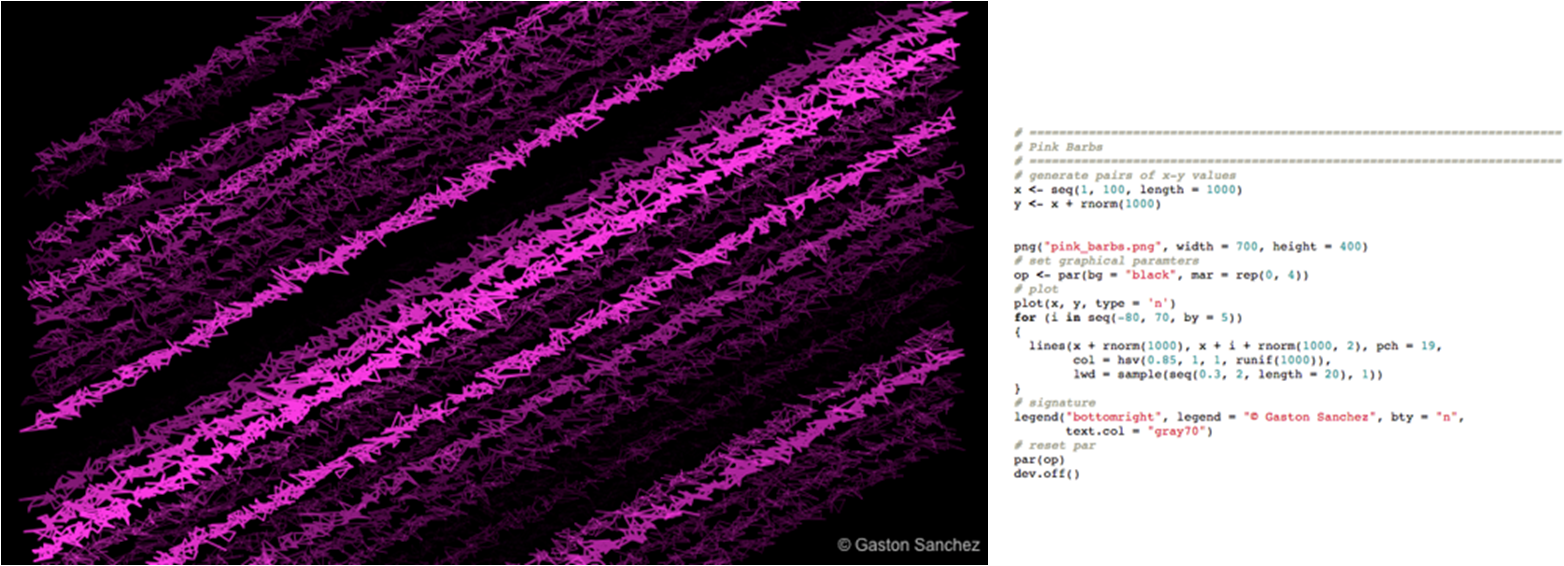
\includegraphics{../external/images/funR_5_aRt_pink_combo.png}

\end{frame}

\end{document}
